\chapter{Ventanas}\label{cap:ventanas}

La transformada de Fourier de tiempo corto (STFT) no analiza una señal completa, sino fragmentos
de ella:
\[
  \chi(m,k)=\sum_{n=0}^{L-1}x[n+mH]\,w[n]\,\e^{-2\pi\iu kn/N}.
\]
Es tentador ver la ventana $w$ como un detalle de implementación: una función que vale entre $0$ y
$1$ y que ``suaviza los cortes''. En este capítulo mostramos que es mucho más que eso.
\textbf{La ventana determina cómo se ve cada componente del sonido en el espectrograma}, y por lo
tanto qué tan limpia puede ser una selección.

A lo largo del capítulo, $L$ es el largo de la ventana (en muestras), $N\ge L$ el tamaño de la
FFT, $H$ el salto entre ventanas y $\Fs$ la frecuencia de muestreo. Para una sucesión finita
$w[0],\dots,w[L-1]$ escribimos su transformada de Fourier en tiempo discreto (TFTD) como
\[
  W(\theta)=\sum_{n=0}^{L-1}w[n]\,\e^{-\iu\theta n},\qquad \theta\in[-\pi,\pi),
\]
donde $\theta$ es la frecuencia angular normalizada (radianes por muestra). Un \emph{bin} es la
separación entre coeficientes de una DFT de tamaño $N$: $2\pi/N$ en $\theta$, o $\Fs/N$ en
hertz. Las medidas de este capítulo se dan en bins con $N=L$, para que no dependan del tamaño.

\section{Cortar es multiplicar}

Tomar el fragmento $m$ de una señal y multiplicarlo por la ventana produce la sucesión
$x_m[n]=x[n+mH]\,w[n]$. La propiedad fundamental es que \emph{multiplicar en el tiempo equivale
a convolucionar en la frecuencia}.

\begin{proposicion}[Teorema de modulación]\label{prop:modulacion}
Si $y[n]=x[n]\,w[n]$, con $x$ de energía finita y $w$ de soporte finito, entonces
\[
  Y(\theta)=\frac{1}{2\pi}\int_{-\pi}^{\pi}X(\varphi)\,W(\theta-\varphi)\dd\varphi .
\]
\end{proposicion}

\begin{proof}
Por la fórmula de inversión de la TFTD, $x[n]=\frac{1}{2\pi}\int_{-\pi}^{\pi}X(\varphi)\e^{\iu\varphi n}\dd\varphi$.
Sustituyendo en $Y(\theta)=\sum_n x[n]w[n]\e^{-\iu\theta n}$ e intercambiando la suma finita con la
integral,
\[
  Y(\theta)=\frac{1}{2\pi}\int_{-\pi}^{\pi}X(\varphi)\sum_{n}w[n]\e^{-\iu(\theta-\varphi)n}\dd\varphi
           =\frac{1}{2\pi}\int_{-\pi}^{\pi}X(\varphi)\,W(\theta-\varphi)\dd\varphi. \qedhere
\]
\end{proof}

La consecuencia más importante para nosotros aparece al aplicar la proposición a una sola
parcial.

\begin{corolario}\label{cor:parcial}
Si $x[n]=A\cos(\theta_0 n+\phi)$, el fragmento ventaneado tiene espectro
\[
  X_m(\theta)=\frac{A}{2}\Bigl(\e^{\iu\phi_m}\,W(\theta-\theta_0)+\e^{-\iu\phi_m}\,W(\theta+\theta_0)\Bigr),
  \qquad \phi_m=\phi+\theta_0 mH .
\]
\end{corolario}

Es decir: \textbf{una parcial pura no se ve como una línea, sino como una copia de $W$ centrada en
su frecuencia}. La forma de la transformada de la ventana es, literalmente, la forma que tiene
cada armónico en el espectrograma.

\begin{ejemplo}[La ventana rectangular]
Para $w[n]=1$ en $0\le n<L$, la suma geométrica da el \emph{núcleo de Dirichlet}
\[
  W_R(\theta)=\sum_{n=0}^{L-1}\e^{-\iu\theta n}=\frac{1-\e^{-\iu\theta L}}{1-\e^{-\iu\theta}}
           =\e^{-\iu\theta(L-1)/2}\,\frac{\sin(L\theta/2)}{\sin(\theta/2)} .
\]
Su módulo vale $L$ en $\theta=0$ y se anula por primera vez en $\theta=2\pi/L$, a un bin.
Después oscila con \emph{lóbulos laterales} que decaen como $1/|\theta|$; el mayor está a
$-13.3\dB$. ``No usar ventana'' es usar esta, que es la peor de todas para aislar parciales.
\end{ejemplo}

\section{Fuga espectral y resolución}

Que cada parcial se vea como una copia de $W$ tiene dos efectos, y ambos dependen solo de la forma
de la ventana:
\begin{itemize}
  \item \textbf{Resolución.} Dos parciales más cercanas que el ancho del \emph{lóbulo principal}
        de $W$ se funden en una sola mancha.
  \item \textbf{Fuga espectral.} Los \emph{lóbulos laterales} reparten energía de cada parcial en
        frecuencias donde no hay nada, y pueden tapar parciales débiles cercanas.
\end{itemize}
Con $L$ fijo, no se pueden mejorar ambas a la vez: las ventanas con lóbulos laterales bajos tienen
lóbulos principales anchos, y viceversa. La \cref{fig:fuga} muestra el efecto con dos tonos: uno
fuerte, que cae justo entre dos bins, y otro $60\dB$ más débil, a 13.5 bins de distancia.

\begin{figure}[ht]
  \centering
  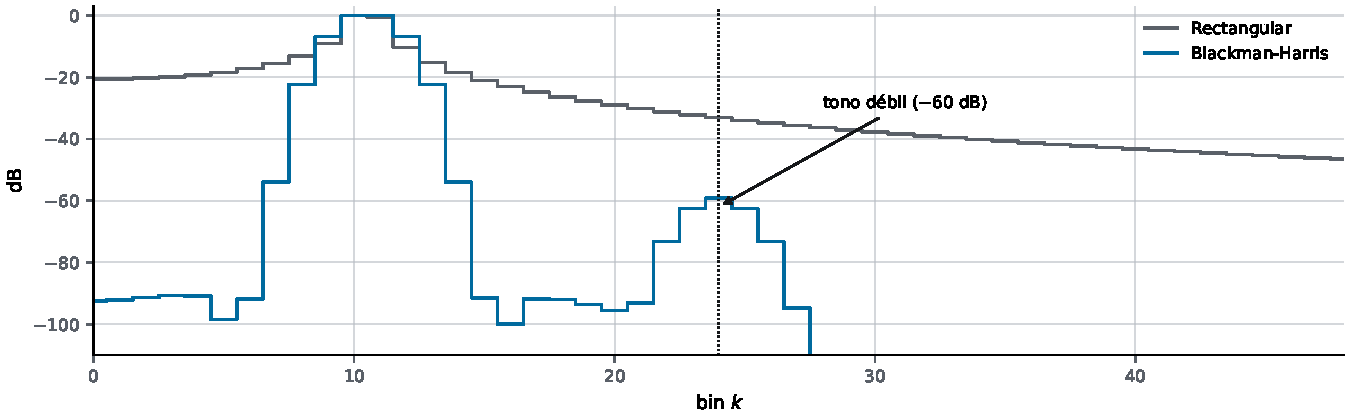
\includegraphics[width=\linewidth]{generated/fuga.pdf}
  \caption{Un tono entre los bins 10 y 11, más un tono de $-60\dB$ en el bin 24. Con la ventana
  rectangular, la fuga del tono fuerte cubre al débil. Con Blackman-Harris, el débil es
  perfectamente visible.}
  \label{fig:fuga}
\end{figure}

\begin{estudio}
Si en Fourierizer seleccionas una parcial débil que está junto a una muy fuerte, por ejemplo el
brillo de una campana junto a su fundamental, con una ventana de lóbulos laterales altos tu
selección también ``atrapa'' energía de la parcial fuerte. Al sintetizar, oirás restos de lo que
querías dejar fuera. Para selecciones finas entre parciales, usa ventanas de lóbulos bajos
(Blackman-Harris, Kaiser con $\beta$ alto).
\end{estudio}

\section{Las medidas de una ventana}

Para comparar ventanas de forma objetiva usamos cuatro medidas clásicas~\cite{harris1978}.

\begin{definicion}
Sea $w$ una ventana de largo $L$ y $W$ su TFTD. Con frecuencias medidas en bins ($2\pi/L$):
\begin{enumerate}
  \item El \emph{primer nulo} es la menor frecuencia positiva donde $|W|$ alcanza un mínimo local.
        Mide la mitad del ancho del lóbulo principal.
  \item El \emph{nivel máximo de lóbulo lateral} es $\max_{\theta>\theta_{\text{nulo}}}20\log_{10}\bigl(|W(\theta)|/|W(0)|\bigr)$.
  \item El \emph{ancho de banda equivalente de ruido} es
        $\displaystyle \mathrm{ENBW}=\frac{L\sum_n w[n]^2}{\bigl(\sum_n w[n]\bigr)^2}$.
  \item La \emph{pérdida por festoneo} es $20\log_{10}\bigl(|W(\pi/L)|/|W(0)|\bigr)$: el error de
        amplitud de una parcial que cae exactamente entre dos bins.
\end{enumerate}
\end{definicion}

\begin{proposicion}\label{prop:enbw}
El $\mathrm{ENBW}$ es el ancho, en bins, del filtro rectangular ideal que, con la misma ganancia
máxima que la ventana, deja pasar la misma potencia de ruido blanco.
\end{proposicion}

\begin{proof}
Sea $e[n]$ ruido blanco de varianza $\sigma^2$. La salida de un bin es $Y=\sum_n w[n]e[n]\e^{-2\pi\iu kn/L}$, y por
independencia $\mathbb{E}|Y|^2=\sigma^2\sum_n w[n]^2$. La ganancia de potencia máxima de la ventana
(la de una parcial centrada en el bin) es $|W(0)|^2=\bigl(\sum_n w[n]\bigr)^2$. El ruido blanco
reparte su potencia por igual entre los $L$ bins, así que tiene $\sigma^2/L$ por bin, y un filtro
rectangular de ancho $B$ bins y ganancia $|W(0)|^2$ deja pasar $|W(0)|^2 B\sigma^2/L$. Igualar
ambas potencias da $B=L\sum w^2/(\sum w)^2$.
\end{proof}

La \cref{tab:ventanas} resume las siete ventanas de Fourierizer y la \cref{fig:ventanas} muestra
sus formas y sus espectros.

\begin{table}[ht]
  \centering\small
  % generated by python/examples/theory_figures.py — do not edit
\begin{tabular}{lrrrr}
\toprule
Ventana & Primer nulo [bins] & Lóbulo lateral máx. [dB] & ENBW [bins] & Festoneo [dB] \\
\midrule
Rectangular & 1.00 & -13.3 & 1.00 & -3.92 \\
Hann & 2.00 & -31.5 & 1.50 & -1.42 \\
Hamming & 2.00 & -42.6 & 1.36 & -1.75 \\
Blackman-Harris & 4.00 & -92.0 & 2.00 & -0.83 \\
Kaiser ($\beta=8$) & 2.73 & -58.7 & 1.67 & -1.18 \\
Gauss ($\sigma=0.4$) & 3.20 & -43.2 & 1.45 & -1.58 \\
Flat-top & 5.00 & -91.5 & 3.77 & -0.01 \\
\bottomrule
\end{tabular}

  \caption{Medidas de las ventanas de Fourierizer (calculadas con el motor de referencia, $L=128$,
  sobremuestreo $\times256$). Coinciden con los valores clásicos de~\cite{harris1978}.}
  \label{tab:ventanas}
\end{table}

\begin{figure}[ht]
  \centering
  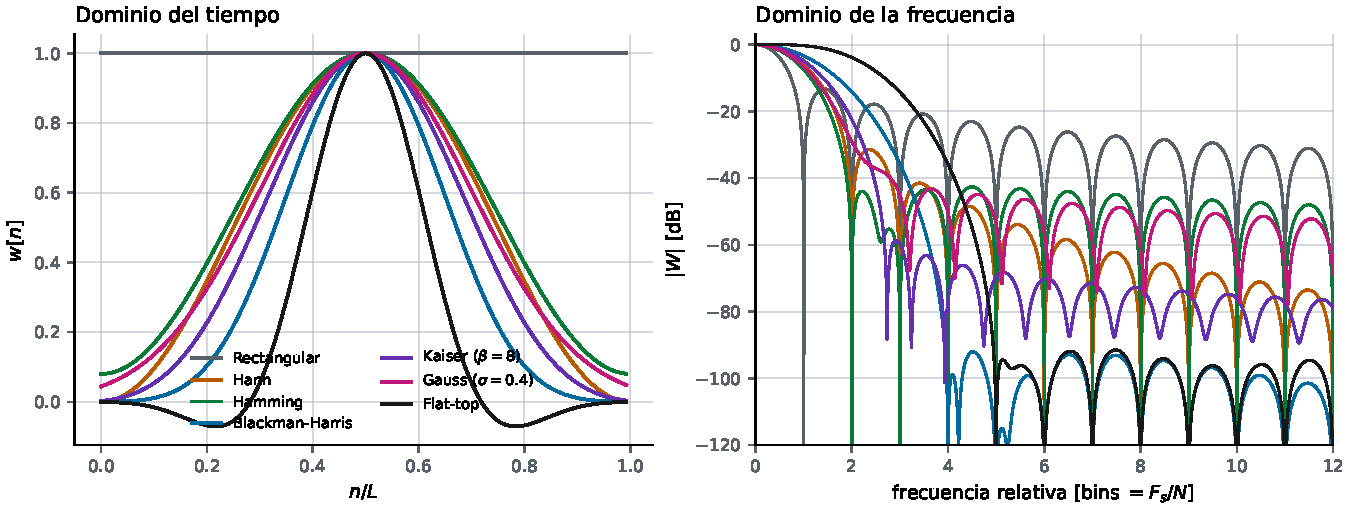
\includegraphics[width=\linewidth]{generated/ventanas.pdf}
  \caption{Las siete ventanas: forma (izquierda) y módulo de su transformada en dB (derecha).}
  \label{fig:ventanas}
\end{figure}

\section{La familia de cosenos generalizados}

Cinco de las siete ventanas son sumas de cosenos:
\begin{equation}\label{eq:cosenos}
  w[n]=\sum_{k=0}^{K}(-1)^k a_k\cos\!\Bigl(\frac{2\pi kn}{L}\Bigr),\qquad 0\le n<L .
\end{equation}

\begin{center}\small
\begin{tabular}{lcl}
\toprule
Ventana & $K$ & coeficientes $a_k$ \\
\midrule
Rectangular & 0 & $1$ \\
Hann & 1 & $\tfrac12,\ \tfrac12$ \\
Hamming & 1 & $0.54,\ 0.46$ \\
Blackman-Harris (4 términos) & 3 & $0.35875,\ 0.48829,\ 0.14128,\ 0.01168$ \\
Flat-top (5 términos) & 4 & $0.21558,\ 0.41663,\ 0.27726,\ 0.08358,\ 0.00695$ \\
\bottomrule
\end{tabular}
\end{center}

\begin{proposicion}\label{prop:suma-dirichlet}
La transformada de una ventana \eqref{eq:cosenos} es una suma de núcleos de Dirichlet desplazados:
\[
  W(\theta)=a_0W_R(\theta)+\sum_{k=1}^{K}(-1)^k\frac{a_k}{2}\Bigl(W_R\bigl(\theta-\tfrac{2\pi k}{L}\bigr)+W_R\bigl(\theta+\tfrac{2\pi k}{L}\bigr)\Bigr).
\]
\end{proposicion}

\begin{proof}
Escribimos $\cos(2\pi kn/L)=\tfrac12(\e^{2\pi\iu kn/L}+\e^{-2\pi\iu kn/L})$. Multiplicar una sucesión
por $\e^{\iu\theta_k n}$ desplaza su TFTD en $\theta_k$, y la ventana es esa suma multiplicada por la
rectangular. Se concluye por linealidad.
\end{proof}

Esta es la idea detrás del diseño de estas ventanas: se eligen los $a_k$ para que los lóbulos
laterales de los núcleos desplazados \emph{se cancelen entre sí}. Hann lo logra de forma ``suave''.
Como su extensión periódica es continua y con derivada continua, sus lóbulos decaen como
$|\theta|^{-3}$ ($-18\dB$ por octava). Hamming sacrifica esa suavidad: deja un pequeño escalón en
los extremos ($w[0]=0.08$) a cambio de cancelar casi por completo el primer lóbulo lateral
($-42.6\dB$), aunque los siguientes decaen solo como $|\theta|^{-1}$. Blackman-Harris usa cuatro
términos para bajar todos los lóbulos por debajo de $-92\dB$, a costa de un lóbulo principal del
doble de ancho que Hann. Flat-top se diseña con otro objetivo: que la cima del lóbulo principal
sea plana, de modo que la pérdida por festoneo sea prácticamente cero ($-0.01\dB$). Es la ventana
de medición, la que da la amplitud exacta de una parcial sin importar dónde caiga.

\section{Kaiser: concentración ajustable}

Una pregunta natural: entre todas las sucesiones de largo $L$, ¿cuál concentra la mayor fracción
de su energía en una banda $|\theta|\le\theta_c$? Es decir, ¿cuál maximiza
\[
  \lambda(w)=\frac{\int_{-\theta_c}^{\theta_c}|W(\theta)|^2\dd\theta}{\int_{-\pi}^{\pi}|W(\theta)|^2\dd\theta}\,?
\]
Por Parseval, $\lambda$ es un cociente de Rayleigh $w^{\mathsf T}Aw/w^{\mathsf T}w$ con
$A_{nm}=\frac{\sin\theta_c(n-m)}{\pi(n-m)}$, así que el óptimo es el vector propio principal de $A$:
la \emph{sucesión esferoidal prolata discreta} de Slepian~\cite{slepian1978}. Kaiser encontró una
aproximación cerrada excelente~\cite{kaiser1974}:
\[
  w[n]=\frac{I_0\!\bigl(\beta\sqrt{1-(2n/L-1)^2}\bigr)}{I_0(\beta)},
\]
donde $I_0$ es la función de Bessel modificada de orden cero. El parámetro $\beta$ recorre todo el
compromiso entre resolución y fuga: con $\beta=0$ se obtiene la rectangular, y al crecer $\beta$
los lóbulos laterales bajan mientras el principal se ensancha. Con $\beta=8$, el valor por defecto
de Fourierizer, se obtienen $-58.7\dB$ con el primer nulo a $2.73$ bins.

\section{Gauss y el principio de incertidumbre}

En el continuo, para $g\in L^2(\R)$ con $\|g\|=1$ y $\hat g(\nu)=\int g(t)\e^{-2\pi\iu\nu t}\dd t$,
definimos las dispersiones $\sigma_t^2=\int(t-\bar t)^2|g(t)|^2\dd t$ y
$\sigma_\nu^2=\int(\nu-\bar\nu)^2|\hat g(\nu)|^2\dd\nu$.

\begin{teorema}[Heisenberg–Gabor]
$\sigma_t\,\sigma_\nu\ge\dfrac{1}{4\pi}$, con igualdad si y solo si $g$ es una gaussiana
(trasladada y modulada).
\end{teorema}

La demostración usual aplica Cauchy–Schwarz a $\langle tg,\,g'\rangle$; puede consultarse
en~\cite{grochenig2001}. Este teorema es la versión precisa de ``no se puede tener todo'':
ninguna ventana está a la vez muy concentrada en tiempo y en frecuencia, y la gaussiana es la que
mejor reparte el compromiso. En el mundo discreto hay que truncarla a $L$ muestras, y el corte
reintroduce lóbulos laterales ($-43.2\dB$ con $\sigma=0.4$). Un $\sigma$ menor reduce el corte
pero ensancha el lóbulo principal. Volveremos a este teorema en el \cref{cap:stft}, donde fija el
límite de lo que puede ``ver'' un espectrograma.

\section{Ventanas periódicas y el solapamiento constante}

Una ventana \emph{simétrica} muestrea $f(n/(L-1))$; una \emph{periódica} muestrea $f(n/L)$, es
decir, un periodo de una función de periodo $L$. Fourierizer usa siempre ventanas periódicas.
La razón es el siguiente resultado, que justifica los saltos ``clásicos''.

\begin{proposicion}[COLA de los cosenos generalizados]\label{prop:cola}
Sea $w$ periódica de la forma \eqref{eq:cosenos} con $K$ términos de coseno, extendida por cero
fuera de $[0,L)$. Si $L=RH$ con $R$ entero y $R>K$, entonces
\[
  \sum_{m\in\Z}w[n-mH]=R\,a_0\qquad\text{para todo } n .
\]
\end{proposicion}

\begin{proof}
Fijemos $n$ y sea $n_0=n\bmod H$. Las ventanas que cubren a $n$ son exactamente $R$ consecutivas,
y en ellas $n-mH$ recorre $n_0+jH$ con $j=0,\dots,R-1$. Para cada $k\ge1$,
\[
  \sum_{j=0}^{R-1}\cos\Bigl(\frac{2\pi k(n_0+jL/R)}{L}\Bigr)=\mathrm{Re}\Bigl(\e^{2\pi\iu kn_0/L}\sum_{j=0}^{R-1}\e^{2\pi\iu kj/R}\Bigr)=0,
\]
porque la suma geométrica de raíces $R$-ésimas de la unidad se anula siempre que $R\nmid k$, y
$1\le k\le K<R$. Solo sobrevive el término $k=0$, que aporta $R\,a_0$.
\end{proof}

\begin{corolario}
Son COLA: Hann y Hamming con $H\le L/2$; Blackman-Harris con $H\le L/4$; flat-top con $H\le L/5$
(siempre con $L/H$ entero). Kaiser y Gauss no son sumas de cosenos y solo son COLA de forma
aproximada.
\end{corolario}

\begin{observacion}
La inversa de mínimos cuadrados que usa Fourierizer (\cref{cap:stft}) no necesita COLA. Solo
necesita que $\sum_m w[n-mH]^2$ no se anule (NOLA), así que \emph{cualquier} ventana sirve con un
salto razonable. COLA importa para que las modificaciones del espectro (las máscaras) se
reconstruyan sin modulaciones de amplitud entre ventanas, y por eso los valores por defecto de
cada ventana usan saltos COLA.
\end{observacion}

\section{Rellenar con ceros no mejora la resolución}

Usar $N>L$ (\emph{zero-padding}) añade ceros a cada fragmento antes de la FFT. La DFT de tamaño $N$
de un fragmento rellenado vale $W$ evaluada en $\theta_k=2\pi k/N$: \emph{son más muestras de la
misma curva}. El espectrograma se dibuja más fino y la posición de los picos se estima con más
precisión, pero el ancho del lóbulo principal (la resolución real) no cambia. Ese ancho lo fijan
$L$ y la forma de la ventana.

\begin{ejemplo}[¿Qué $L$ necesito para separar dos parciales?]
Dos parciales separadas por $\Delta f$ se distinguen si el primer nulo de la ventana, en hertz,
es menor que $\Delta f$:
\[
  \nu_{\text{nulo}}\cdot\frac{\Fs}{L}\le\Delta f\quad\Longleftrightarrow\quad L\ge\frac{\nu_{\text{nulo}}\,\Fs}{\Delta f}.
\]
Con $\Fs=48\,000\Hz$ y armónicos separados por $\Delta f=100\Hz$ (una nota cerca de Sol$_2$),
Hann ($\nu_{\text{nulo}}=2$) necesita $L\ge960$ muestras ($20$ ms). Blackman-Harris
($\nu_{\text{nulo}}=4$) necesita $L\ge1920$ ($40$ ms).
\end{ejemplo}

\begin{estudio}
\textbf{Qué ventana elegir en Fourierizer.}
\begin{itemize}
  \item \emph{Percusiones (kicks, snares, hats).} Ventana corta (L de 256 a 1024) y Hann. Lo
        importante es el ataque; la resolución en frecuencia casi no importa.
  \item \emph{Pads, cuerdas y notas sostenidas.} Ventana larga (L de 4096 o más) con
        Blackman-Harris o Kaiser con $\beta$ entre 8 y 12. Los armónicos quedan bien separados y
        con poca fuga, ideal para seleccionarlos uno por uno.
  \item \emph{Campanas y sonidos inarmónicos con parciales débiles.} Blackman-Harris: sus lóbulos
        de $-92\dB$ dejan ver todo.
  \item \emph{Medir niveles exactos.} Flat-top. Es mala para separar, pero la más honesta en
        amplitud.
  \item \emph{Como efecto.} La rectangular ``mancha'' cada parcial a lo ancho del espectro. Es
        una mala ventana de análisis, pero puede ser una textura interesante.
\end{itemize}
Subir $N$ solo mejora el dibujo. Para separar notas cercanas hay que subir $L$, y el precio es
emborronar los ataques. En el \cref{cap:multirresolucion} veremos cómo evitar ese dilema usando
ventanas distintas por banda.
\end{estudio}
